\documentclass{article}\usepackage[]{graphicx}\usepackage[]{color}
%% maxwidth is the original width if it is less than linewidth
%% otherwise use linewidth (to make sure the graphics do not exceed the margin)
\makeatletter
\def\maxwidth{ %
  \ifdim\Gin@nat@width>\linewidth
    \linewidth
  \else
    \Gin@nat@width
  \fi
}
\makeatother

\definecolor{fgcolor}{rgb}{0.345, 0.345, 0.345}
\newcommand{\hlnum}[1]{\textcolor[rgb]{0.686,0.059,0.569}{#1}}%
\newcommand{\hlstr}[1]{\textcolor[rgb]{0.192,0.494,0.8}{#1}}%
\newcommand{\hlcom}[1]{\textcolor[rgb]{0.678,0.584,0.686}{\textit{#1}}}%
\newcommand{\hlopt}[1]{\textcolor[rgb]{0,0,0}{#1}}%
\newcommand{\hlstd}[1]{\textcolor[rgb]{0.345,0.345,0.345}{#1}}%
\newcommand{\hlkwa}[1]{\textcolor[rgb]{0.161,0.373,0.58}{\textbf{#1}}}%
\newcommand{\hlkwb}[1]{\textcolor[rgb]{0.69,0.353,0.396}{#1}}%
\newcommand{\hlkwc}[1]{\textcolor[rgb]{0.333,0.667,0.333}{#1}}%
\newcommand{\hlkwd}[1]{\textcolor[rgb]{0.737,0.353,0.396}{\textbf{#1}}}%

\usepackage{framed}
\makeatletter
\newenvironment{kframe}{%
 \def\at@end@of@kframe{}%
 \ifinner\ifhmode%
  \def\at@end@of@kframe{\end{minipage}}%
  \begin{minipage}{\columnwidth}%
 \fi\fi%
 \def\FrameCommand##1{\hskip\@totalleftmargin \hskip-\fboxsep
 \colorbox{shadecolor}{##1}\hskip-\fboxsep
     % There is no \\@totalrightmargin, so:
     \hskip-\linewidth \hskip-\@totalleftmargin \hskip\columnwidth}%
 \MakeFramed {\advance\hsize-\width
   \@totalleftmargin\z@ \linewidth\hsize
   \@setminipage}}%
 {\par\unskip\endMakeFramed%
 \at@end@of@kframe}
\makeatother

\definecolor{shadecolor}{rgb}{.97, .97, .97}
\definecolor{messagecolor}{rgb}{0, 0, 0}
\definecolor{warningcolor}{rgb}{1, 0, 1}
\definecolor{errorcolor}{rgb}{1, 0, 0}
\newenvironment{knitrout}{}{} % an empty environment to be redefined in TeX

\usepackage{alltt}
\usepackage{natbib}
\usepackage[unicode=true]{hyperref}
\usepackage{geometry}
\geometry{tmargin=1in,bmargin=1in,lmargin=1in,rmargin=1in}
\setlength\parindent{0pt}
\IfFileExists{upquote.sty}{\usepackage{upquote}}{}
\begin{document} 
\title{Stat243 PS3}
\author{Meng Wang, SID: 21706745}
\date{Septembre 27, 2015}

\maketitle


\begin{document}
\section{Problem 2}
\subsection{(a)}

There are two problems we need to solve here: the first problem is to extract all the links from the downloaded file; the second problem is to find out among the links that it is the first debate of a specific years we are interested in. Let us deal with these two problems one by one.

The first problem is straightforward. Using the content on the material of unit3, we could download the data and parse, and exact the urls in the parsed file. The links are saved in \textit{links}

\begin{knitrout}
\definecolor{shadecolor}{rgb}{0.969, 0.969, 0.969}\color{fgcolor}\begin{kframe}
\begin{alltt}
 \hlkwd{library}\hlstd{(XML)}
 \hlkwd{library}\hlstd{(curl)}

 \hlcom{# download all content on the page}
 \hlstd{URL} \hlkwb{<-} \hlstr{"http://www.debates.org/index.php?page=debate-transcripts"}\hlstd{;}
 \hlstd{page} \hlkwb{<-} \hlkwd{htmlParse}\hlstd{(URL);}

 \hlcom{# extract the all the links on page for future use}
 \hlstd{allSpeech} \hlkwb{<-} \hlkwd{getNodeSet}\hlstd{(page,} \hlstr{"//a[@title]"}\hlstd{)}
 \hlstd{links} \hlkwb{<-} \hlkwd{sapply}\hlstd{(allSpeech, xmlGetAttr,} \hlstr{"href"}\hlstd{)}
\end{alltt}
\end{kframe}
\end{knitrout}

Since the titles on the website debate contain the key word  \lq First\rq . What we need to do for the second problem is, to transfer the data download to string type and find the index of the strings which matches the keyword \lq First\rq and the number of year. The position are stored in the \textit{index} 

\begin{knitrout}
\definecolor{shadecolor}{rgb}{0.969, 0.969, 0.969}\color{fgcolor}\begin{kframe}
\begin{alltt}
 \hlcom{# save the XML as string for keyword matching}
 \hlstd{stringSpeech} \hlkwb{<-} \hlkwd{xpathSApply}\hlstd{(page,} \hlstr{"//a[@title]"}\hlstd{,saveXML)}

 \hlcom{# find the index that contains key word "First" and }
 \hlstd{years} \hlkwb{<-} \hlkwd{c}\hlstd{(}\hlstr{"1996"}\hlstd{,} \hlstr{"2000"}\hlstd{,} \hlstr{"2004"}\hlstd{,} \hlstr{"2008"}\hlstd{,} \hlstr{"2012"}\hlstd{)}

 \hlcom{# function that returns the index of the year}
 \hlstd{findIndex} \hlkwb{<-} \hlkwa{function}\hlstd{(}\hlkwc{year}\hlstd{,} \hlkwc{speechstr}\hlstd{=stringSpeech)\{}
   \hlkwd{intersect}\hlstd{(}\hlkwd{grep}\hlstd{(year, speechstr),} \hlkwd{grep}\hlstd{(}\hlstr{"First"}\hlstd{, speechstr))}
 \hlstd{\}}
 \hlcom{# find the index for every years' first speech}
 \hlstd{index} \hlkwb{<-}\hlkwd{sapply}\hlstd{(years, findIndex)}
\end{alltt}
\end{kframe}
\end{knitrout}

The results are stored in \lq index\rq and the element is names integer. So we could find the link and the content by using the year directly. For example, we want the first speech in year 2006, here is the results,

\begin{knitrout}
\definecolor{shadecolor}{rgb}{0.969, 0.969, 0.969}\color{fgcolor}\begin{kframe}
\begin{alltt}
 \hlstd{links[index[}\hlstr{"1996"}\hlstd{]]}
\end{alltt}
\begin{verbatim}
## [1] "http://www.debates.org/index.php?page=october-6-1996-debate-transcript"
\end{verbatim}
\end{kframe}
\end{knitrout}

\subsection{(b)}
This part is very straight forward. Exact the debate part first and then replace the nextline in HTML to the corresponding ones in the text file. Here is the code.

\begin{knitrout}
\definecolor{shadecolor}{rgb}{0.969, 0.969, 0.969}\color{fgcolor}\begin{kframe}
\begin{alltt}
 \hlcom{# function that returns the debate in txt file format}
 \hlcom{# input: string year = "2000"}
 \hlcom{# output: string contains the debate content}
 \hlstd{extractTXT} \hlkwb{<-} \hlkwa{function}\hlstd{(}\hlkwc{year} \hlstd{=} \hlstr{"2012"}\hlstd{)\{}
   \hlcom{# Parse the document}
   \hlstd{debate} \hlkwb{<-} \hlkwd{htmlParse}\hlstd{(links[index[year]])}
  \hlcom{# extract the debate part}
  \hlstd{content}  \hlkwb{<-} \hlkwd{xpathSApply}\hlstd{(debate,} \hlstr{'//div[@id="content-sm"]'}\hlstd{,saveXML)}
  \hlcom{# change format from HTML to txt}
  \hlstd{content} \hlkwb{<-} \hlkwd{gsub}\hlstd{(}\hlstr{"<br>|<br/>"}\hlstd{,}\hlstr{"\textbackslash{}n"}\hlstd{, content)}
  \hlstd{content} \hlkwb{<-} \hlkwd{gsub}\hlstd{(}\hlstr{'<(.*?)>'}\hlstd{,} \hlstr{""}\hlstd{, content)}
  \hlkwd{return}\hlstd{(content)}
\hlstd{\}}
\end{alltt}
\end{kframe}
\end{knitrout}

Extract all the spoken part for each year and put them into \lq spokenDebate\rq .
\begin{knitrout}
\definecolor{shadecolor}{rgb}{0.969, 0.969, 0.969}\color{fgcolor}\begin{kframe}
\begin{alltt}
 \hlstd{spokenDebate} \hlkwb{<-} \hlkwd{sapply}\hlstd{(years, extractTXT)}
 \hlcom{# test }
 \hlcom{# spokenDebate["1996"]}
\end{alltt}
\end{kframe}
\end{knitrout}

\subsection{(c)}
In this part, we are asked to split the who speech and merge them together, so that we have the speech for each candidate for future analysis. The good news is that for lots of the paragraph,  it starts with the speaker's name. So we could easily split the whole speech to paragraph, and scan the paragraphs to see whether there are any speaker's name included or not. This is very straight-forward. The tricky part of the work is however, how to know which speaker those paragraphs which do not have any speaker's name belongs to. Naturally we know it belongs to the speaker of the last paragraph with a speaker's name. In summary, the algorithm to this problem is, first, split the speech to paragraphs; Secondly, loop through the paragraphs. For each paragraph, check whether contains the name of the speaker or not. If it contains the speaker's name, we should save it. If it does not, also it does not belongs to any speaker's, we should check who the last speaker is. If the last speaker is the one we are looking for, then we should save this paragraph too. If it is not, we should continue looping. Here is the code.

First, we need a function to find out all the speakers of that year,
\begin{knitrout}
\definecolor{shadecolor}{rgb}{0.969, 0.969, 0.969}\color{fgcolor}\begin{kframe}
\begin{alltt}
 \hlcom{## function used to find the candidate by splitting the string to words}
 \hlcom{## input: year = "1996", data = spokenDebate}
 \hlcom{## output: name of the speakers}
 \hlstd{findSpeaker} \hlkwb{<-} \hlkwa{function}\hlstd{(}\hlkwc{year} \hlstd{,} \hlkwc{data}\hlstd{=spokenDebate)\{}
  \hlcom{# change the '\textbackslash{}n' to space for word splitting}
  \hlstd{text_no_newline} \hlkwb{<-} \hlkwd{gsub}\hlstd{(}\hlstr{"\textbackslash{}n"}\hlstd{,} \hlstr{" "}\hlstd{, data[year])}
  \hlcom{# split the word}
  \hlstd{split_word} \hlkwb{<-} \hlkwd{strsplit}\hlstd{(text_no_newline,}\hlstr{" "}\hlstd{)[[}\hlnum{1}\hlstd{]]}
  \hlcom{# find the names which has the pattern: all capital words followed by a :}
  \hlstd{speaker} \hlkwb{<-} \hlstd{split_word[}\hlkwd{grep}\hlstd{(}\hlstr{"[[:upper:]]:"}\hlstd{, split_word)]}
  \hlstd{speaker} \hlkwb{<-} \hlkwd{unique}\hlstd{(speaker)}
  \hlkwd{return}\hlstd{(speaker)}
 \hlstd{\}}
\end{alltt}
\end{kframe}
\end{knitrout}

These are the speakers for 1996, as a test for the function
\begin{knitrout}
\definecolor{shadecolor}{rgb}{0.969, 0.969, 0.969}\color{fgcolor}\begin{kframe}
\begin{alltt}
 \hlcom{# test }
 \hlkwd{findSpeaker}\hlstd{(}\hlstr{"1996"}\hlstd{)}
\end{alltt}
\begin{verbatim}
## [1] "LEHRER:"  "CLINTON:" "DOLE:"
\end{verbatim}
\end{kframe}
\end{knitrout}

Next, we need a function that can do the loop we discussed previously and merge all the paragraphs for a speaker at a specific year. Another little function is required to check whether this paragraph belongs to any speaker of this year or not. Here are the codes,

\begin{knitrout}
\definecolor{shadecolor}{rgb}{0.969, 0.969, 0.969}\color{fgcolor}\begin{kframe}
\begin{alltt}
\hlcom{## function: find whether this string belongs to any speaker or not}
\hlstd{checkOwner} \hlkwb{<-} \hlkwa{function}\hlstd{(}\hlkwc{allSpeakers}\hlstd{,} \hlkwc{str}\hlstd{)\{}
  \hlstd{check} \hlkwb{=} \hlnum{0}\hlstd{;}
  \hlkwa{for} \hlstd{(i} \hlkwa{in} \hlnum{1}\hlopt{:}\hlkwd{length}\hlstd{(allSpeakers))\{}
    \hlkwa{if} \hlstd{(}\hlkwd{grepl}\hlstd{(allSpeakers[i], str)) check} \hlkwb{=} \hlstd{check}\hlopt{+}\hlnum{1}
  \hlstd{\}}
  \hlkwd{return}\hlstd{(check)}
\hlstd{\}}

\hlcom{## function: exact the speech given by each candidate}
\hlcom{## Input: speaker = "CLINTON:", yera = "2006", data = spokenDebate}
\hlcom{## Output: speech of the speaker}
\hlstd{speakerSpeech} \hlkwb{<-} \hlkwa{function}\hlstd{(}\hlkwc{speaker}\hlstd{,} \hlkwc{year}\hlstd{,} \hlkwc{data}\hlstd{=spokenDebate)\{}
 \hlcom{# fisrst get rid of "Laughter" and "Applause"}
 \hlstd{spokenData} \hlkwb{<-} \hlkwd{gsub}\hlstd{(}\hlstr{"Laughter"}\hlstd{,} \hlstr{""}\hlstd{, data[year])}
 \hlstd{spokenData} \hlkwb{<-} \hlkwd{gsub}\hlstd{(}\hlstr{"Applause"}\hlstd{,} \hlstr{""}\hlstd{, spokenData)}
 \hlcom{# split the string into paragraphs}
 \hlstd{split_para} \hlkwb{<-} \hlkwd{strsplit}\hlstd{(spokenData[year],}\hlstr{"\textbackslash{}n"}\hlstd{)[[}\hlnum{1}\hlstd{]]}
 \hlcom{# remove the blank paragraph}
 \hlstd{split_para} \hlkwb{<-} \hlstd{split_para[}\hlopt{!} \hlstd{split_para} \hlopt{==} \hlstr{""}\hlstd{]}
 \hlcom{# for loop to go throught all the paragraphs}
 \hlstd{speak_talk} \hlkwb{=} \hlnum{0} \hlcom{# 1 means this paragraph belong to the speaker}
 \hlstd{k} \hlkwb{=} \hlnum{1}
 \hlstd{speak_speech} \hlkwb{<-} \hlkwd{c}\hlstd{(}\hlstr{""}\hlstd{)}
 \hlkwa{for} \hlstd{(para_num} \hlkwa{in} \hlnum{1}\hlopt{:}\hlkwd{length}\hlstd{(split_para))\{}
   \hlkwa{if} \hlstd{(}\hlkwd{grepl}\hlstd{(speaker, split_para[para_num]))\{}
     \hlcom{# this paragrah does belongs to the speaker}
     \hlstd{speak_talk} \hlkwb{=} \hlnum{1}\hlstd{;}
     \hlstd{speak_speech[k]} \hlkwb{<-} \hlstd{split_para[para_num]}
     \hlstd{k} \hlkwb{=} \hlstd{k}\hlopt{+}\hlnum{1}
   \hlstd{\}}
   \hlkwa{else if}\hlstd{(}\hlkwd{checkOwner}\hlstd{(}\hlkwd{findSpeaker}\hlstd{(year), split_para[para_num])} \hlopt{==} \hlnum{0}\hlstd{)\{}
     \hlkwa{if} \hlstd{(speak_talk} \hlopt{==} \hlnum{1}\hlstd{)}
     \hlstd{\{} \hlcom{# the paragrah is a continuing of the last paragraph}
       \hlstd{speak_speech[k]} \hlkwb{<-} \hlstd{split_para[para_num]}
       \hlstd{k} \hlkwb{=} \hlstd{k}\hlopt{+}\hlnum{1}
     \hlstd{\}}
   \hlstd{\}}
   \hlkwa{else}\hlstd{\{} \hlcom{# this paragraph belongs to someone else}
     \hlstd{speak_talk} \hlkwb{=} \hlnum{0}
   \hlstd{\}}
 \hlstd{\}}
 \hlcom{# put all paragraph together}
 \hlstd{speak_speech} \hlkwb{<-} \hlkwd{paste}\hlstd{(speak_speech,} \hlkwc{set}\hlstd{=}\hlstr{""}\hlstd{,} \hlkwc{collapse}\hlstd{=}\hlstr{""}\hlstd{)}
 \hlcom{# delete the speaker's name due to duplication}
 \hlstd{speak_speech} \hlkwb{<-} \hlkwd{gsub}\hlstd{(speaker,} \hlstr{""}\hlstd{, speak_speech)}
 \hlkwd{return}\hlstd{(speak_speech)}
\hlstd{\}}
\end{alltt}
\end{kframe}
\end{knitrout}

The code has been tested as following. The result is too long so please run the corresponding R code for the results.
\begin{knitrout}
\definecolor{shadecolor}{rgb}{0.969, 0.969, 0.969}\color{fgcolor}\begin{kframe}
\begin{alltt}
\hlcom{# test}
\hlcom{#speakerSpeech("CLINTON:", "1996")}
\end{alltt}
\end{kframe}
\end{knitrout}


Finally, we could loop through all the speakers with a year and split the debate of that year to several speakers. For efficiency, we use \lq sapply\rq .
\begin{knitrout}
\definecolor{shadecolor}{rgb}{0.969, 0.969, 0.969}\color{fgcolor}\begin{kframe}
\begin{alltt}
\hlcom{# function find all the speeches for one year only}
\hlstd{OneYear_SpeakerSpeech} \hlkwb{<-} \hlkwa{function}\hlstd{(}\hlkwc{one_year}\hlstd{,} \hlkwc{data} \hlstd{= spokenDebate)\{}
  \hlkwd{return} \hlstd{(}\hlkwd{sapply}\hlstd{(}\hlkwd{findSpeaker}\hlstd{(one_year), speakerSpeech,} \hlkwc{year} \hlstd{= one_year))}
\hlstd{\}}
\end{alltt}
\end{kframe}
\end{knitrout}

Since the result are stored characteristically, we could directly check the speech of a speaker by his/her name, for example
\begin{knitrout}
\definecolor{shadecolor}{rgb}{0.969, 0.969, 0.969}\color{fgcolor}\begin{kframe}
\begin{alltt}
 \hlcom{# test}
 \hlstd{speech1996} \hlkwb{<-} \hlkwd{OneYear_SpeakerSpeech}\hlstd{(}\hlstr{"1996"}\hlstd{)}
 \hlstd{speech1996[}\hlstr{"CLINTON:"}\hlstd{]}
\end{alltt}
\end{kframe}
\end{knitrout}

Then loop through the years we are interested with \lq sapply\rq , and we should have the results.
\begin{knitrout}
\definecolor{shadecolor}{rgb}{0.969, 0.969, 0.969}\color{fgcolor}\begin{kframe}
\begin{alltt}
\hlcom{# all the years, all the speeches by the candidates}
 \hlstd{AllSpeach} \hlkwb{<-} \hlkwd{sapply}\hlstd{(years, OneYear_SpeakerSpeech)}
\end{alltt}
\end{kframe}
\end{knitrout}

\subsection{(d)}
This part is very straight forward. To split the sentences, we need to replace dot with nextline character. To split the text to words, we replace nextline character to space. Here are the functions and test case.

\begin{knitrout}
\definecolor{shadecolor}{rgb}{0.969, 0.969, 0.969}\color{fgcolor}\begin{kframe}
\begin{alltt}
\hlcom{## function: exact a string to sentences}
\hlstd{splitToSentence} \hlkwb{<-} \hlkwa{function}\hlstd{(}\hlkwc{str_data} \hlstd{= spokenDebate[}\hlstr{"1996"}\hlstd{])\{}
  \hlcom{# change the '.' to "\textbackslash{}n" for sentence splitting}
  \hlstd{text_data} \hlkwb{<-} \hlkwd{gsub}\hlstd{(}\hlstr{"\textbackslash{}\textbackslash{}."}\hlstd{,} \hlstr{"\textbackslash{}n"}\hlstd{, str_data)}
  \hlstd{sentence} \hlkwb{<-} \hlkwd{strsplit}\hlstd{(text_data,} \hlstr{"\textbackslash{}n"}\hlstd{)[[}\hlnum{1}\hlstd{]]}
  \hlcom{# remove empty lines}
  \hlstd{sentence} \hlkwb{<-} \hlstd{sentence[}\hlopt{!}\hlstd{sentence} \hlopt{==} \hlstr{""}\hlstd{]}
  \hlkwd{return}\hlstd{(sentence)}
\hlstd{\}}
\hlcom{# test }
\hlcom{# sentence1996 <- splitToSentence(spokenDebate["1996"])}

\hlcom{## function: extract the words from string}
\hlstd{splitToWord} \hlkwb{<-} \hlkwa{function} \hlstd{(}\hlkwc{str_data} \hlstd{= spokenDebate[}\hlstr{"1996"}\hlstd{])\{}
  \hlstd{text_noline} \hlkwb{<-} \hlkwd{gsub}\hlstd{(}\hlstr{"\textbackslash{}n"}\hlstd{,} \hlstr{" "}\hlstd{, str_data)}
  \hlcom{# split the word}
  \hlstd{split_word} \hlkwb{<-} \hlkwd{strsplit}\hlstd{(text_noline,}\hlstr{" "}\hlstd{)[[}\hlnum{1}\hlstd{]]}
  \hlcom{# remove empty elements}
  \hlstd{split_word} \hlkwb{<-} \hlstd{split_word[}\hlopt{!} \hlstd{split_word} \hlopt{==} \hlstr{""}\hlstd{]}
  \hlkwd{return}\hlstd{(split_word)}
\hlstd{\}}

\hlcom{# test}
\hlcom{#word1996 <- splitToWord(spokenDebate["1996"])}
\end{alltt}
\end{kframe}
\end{knitrout}

\subsection{(e)}
With the function in part(d), we just to count the length of the words splitted from the speech of each candidate, for the number of the words used. For the number of characters, we could use the function \lq nchar\rq in R to compute the length of each word and then sum the length of each word together. Average word length shall be the ratio of the two quantities we calculated. The results are stored in list format. Here is the function,
\begin{knitrout}
\definecolor{shadecolor}{rgb}{0.969, 0.969, 0.969}\color{fgcolor}\begin{kframe}
\begin{alltt}
\hlcom{## function: do the word statistics and return a list of the data}
wordStat <- \hlkwd{function} (candidate, years, data = spokenDebate)\{
\hlcom{ # get the speech for the candidate of that year}
 candSpeech <- \hlkwd{speakerSpeech}(candidate,  years, data)
\hlcom{ # split the speech to words}
 word <- \hlkwd{splitToWord}(candSpeech)
\hlcom{ # count the length of the words}
 word_number <- \hlkwd{length}(word)
\hlcom{ # count the length of each word and sum up}
 char_length <- \hlkwd{sum}(\hlkwd{nchar}(word))
\hlcom{ # get the average}
 ave_word_length = char_length / word_number 
\hlcom{ # put the statistics to a list}
 result <- \hlkwd{list}(WordNumber = word_number, CharLength=char_length, %AveWordLength=ave_word_length)
 \hlkwd{return}(result)
\}
\end{alltt}
\end{kframe}
\end{knitrout}

And here is the result of a test case,
\begin{knitrout}
\definecolor{shadecolor}{rgb}{0.969, 0.969, 0.969}\color{fgcolor}\begin{kframe}
\begin{alltt}
 \hlkwd{wordStat}\hlstd{(}\hlstr{"CLINTON:"}\hlstd{,} \hlstr{"1996"}\hlstd{)}
\end{alltt}
\begin{verbatim}
## $WordNumber
## [1] 7380
## 
## $CharLength
## [1] 33323
## 
## $AveWordLength
## [1] 4.515312
\end{verbatim}
\end{kframe}
\end{knitrout}

Then we loop the function with each candidate of a year, for every year, with \lq sapply\rq , like what we did in last part. Here is the code,
\begin{knitrout}
\definecolor{shadecolor}{rgb}{0.969, 0.969, 0.969}\color{fgcolor}\begin{kframe}
\begin{alltt}
\hlcom{## function: do the word statistics for each candidate for a year}
\hlstd{wordStat_Year} \hlkwb{<-} \hlkwa{function} \hlstd{(}\hlkwc{one_year}\hlstd{,} \hlkwc{data} \hlstd{= spokenDebate)\{}
  \hlcom{# get the speaker of that year}
  \hlstd{candidate} \hlkwb{<-} \hlkwd{findSpeaker}\hlstd{(one_year)}
  \hlcom{# find all the word statistics of the candidates that year}
  \hlstd{word_stat_year} \hlkwb{<-}\hlkwd{sapply}\hlstd{(candidate, wordStat,} \hlkwc{years} \hlstd{= one_year)}
  \hlkwd{return} \hlstd{(word_stat_year)}
\hlstd{\}}

\hlcom{# test}
\hlcom{# wordStat1996 <- wordStat_Year("1996")}
\hlcom{# wordStatAll <- sapply(years, wordStat_Year)}
\end{alltt}
\end{kframe}
\end{knitrout}

Here is the result (I copied it directly from Rstudio, please run the R code)

\begin{knitrout}
\definecolor{shadecolor}{rgb}{0.969, 0.969, 0.969}\color{fgcolor}\begin{kframe}
\begin{alltt}
> wordStatAll
$`1996`
              LEHRER:  CLINTON: DOLE:   
WordNumber    1218     7380     8114    
CharLength    5800     33323    36305   
AveWordLength 4.761905 4.515312 4.474365

$`2000`
              MODERATOR: GORE:    BUSH:   
WordNumber    1688       7208     7451    
CharLength    8056       32310    33132   
AveWordLength 4.772512   4.482519 4.446651

$`2004`
              SPEAKERS: LEHRER: KERRY:   BUSH:   
WordNumber    26        1362    7150     6345    
CharLength    148       6855    31708    28395   
AveWordLength 5.692308  5.03304 4.434685 4.475177

$`2008`
              SPEAKERS: LEHRER:  OBAMA:   MCCAIN: 
WordNumber    52        2797     15358    14392   
CharLength    316       12779    69128    65516   
AveWordLength 6.076923  4.568824 4.501107 4.552251

$`2012`
             SPEAKERS: LEHRER:  OBAMA:   ROMNEY:
WordNumber    11        1962     7341     7860   
CharLength    67        9174     33647    35161  
AveWordLength 6.090909  4.675841 4.583435 4.47341
\end{alltt}
\end{kframe}
\end{knitrout}

Here are some comment: First, it seems that the number of words for each year and each candidate does not change that much, except year 2008 debate between Obama and McCain, which almost twice as long as the other years. While the word length does not change that much at all, for any year and any candidate. Secondly, the number of words for each speaker at the same year, are almost the same. Speaking more words is not directly related with whether he or she will win the election or not.

\subsection{(f)}
For the last part, we just need to use the function in the previous part to split the speech into words, and count the words we are interested in. You may notice I decided to write the code for each word, instead of writing a function to look for each word. Since the code looking for number of words are very short, it does not save me any efforts to make it a function. So I directly write it.
Here is the function to count the words for one speaker of a year. 
\begin{knitrout}
\definecolor{shadecolor}{rgb}{0.969, 0.969, 0.969}\color{fgcolor}\begin{kframe}
\begin{alltt}
\hlcom{## function: do the words counts for a speaker for a specific year}
\hlstd{wordsCount} \hlkwb{<-} \hlkwa{function} \hlstd{(}\hlkwc{speaker}\hlstd{,} \hlkwc{year}\hlstd{,} \hlkwc{data} \hlstd{= spokenDebate)\{}
 \hlcom{# first find the speech by that speaker }
 \hlstd{speech} \hlkwb{<-} \hlkwd{speakerSpeech}\hlstd{(speaker, year,} \hlkwc{data}\hlstd{=spokenDebate)}
 \hlstd{words} \hlkwb{<-} \hlkwd{splitToWord}\hlstd{(speech)}
 \hlstd{num_I} \hlkwb{=} \hlkwd{length}\hlstd{(words[words} \hlopt{==} \hlstr{"I"}\hlstd{])}
 \hlstd{num_we} \hlkwb{=} \hlkwd{length}\hlstd{(words[words} \hlopt{==} \hlstr{"we"}\hlstd{])}
 \hlcom{# number of words contains America/American}
 \hlstd{num_America} \hlkwb{=} \hlkwd{length}\hlstd{(words[}\hlkwd{grep}\hlstd{(}\hlstr{"America"}\hlstd{, words)])}
 \hlcom{# number of words contains democra}
 \hlstd{num_democra} \hlkwb{=} \hlkwd{length}\hlstd{(words[}\hlkwd{grep}\hlstd{(}\hlstr{"democra"}\hlstd{, words)])}
 \hlstd{num_republic} \hlkwb{=} \hlkwd{length}\hlstd{(words[}\hlkwd{grep}\hlstd{(}\hlstr{"republic"}\hlstd{, words)])}
 \hlstd{num_Democrat} \hlkwb{=} \hlkwd{length}\hlstd{(words[}\hlkwd{grep}\hlstd{(}\hlstr{"Democrat"}\hlstd{, words)])}
 \hlstd{num_Republican} \hlkwb{=} \hlkwd{length}\hlstd{(words[}\hlkwd{grep}\hlstd{(}\hlstr{"Republican"}\hlstd{, words)])}
 \hlstd{num_free} \hlkwb{=} \hlkwd{length}\hlstd{(words[(words} \hlopt{==} \hlstr{"free"}\hlstd{)} \hlopt{|} \hlstd{(words} \hlopt{==} \hlstr{"freedom"}\hlstd{)])}
 \hlstd{num_war} \hlkwb{=} \hlkwd{length}\hlstd{(words[words} \hlopt{==} \hlstr{"war"}\hlstd{])}
 \hlstd{num_God} \hlkwb{=} \hlkwd{length}\hlstd{(words[words} \hlopt{==} \hlstr{"God"}\hlstd{])}
 \hlstd{num_GodBless} \hlkwb{=} \hlkwd{length}\hlstd{(words[words} \hlopt{==} \hlstr{"God bless"}\hlstd{])}
 \hlstd{num_Jesus} \hlkwb{=} \hlkwd{length}\hlstd{(words[words} \hlopt{==} \hlstr{"Jesus"} \hlopt{|} \hlstd{words} \hlopt{==} \hlstr{"Christ"} \hlopt{|} \hlstd{words} \hlopt{==} \hlstr{"Christian"}\hlstd{])}
 \hlstd{num_words} \hlkwb{<-} \hlkwd{list}\hlstd{(}\hlkwc{num_I} \hlstd{= num_I,} \hlkwc{num_we} \hlstd{= num_we,} \hlkwc{num_America} \hlstd{= num_we,} \hlkwc{num_democra} \hlstd{= num_democra,}
                   \hlkwc{num_republic} \hlstd{= num_republic,} \hlkwc{num_Democrat}\hlstd{=num_Democrat,} \hlkwc{num_Republican}\hlstd{=num_Republican,}
                   \hlkwc{num_free} \hlstd{= num_free,} \hlkwc{num_war} \hlstd{= num_war,} \hlkwc{num_God} \hlstd{= num_God,} \hlkwc{num_GodBless}\hlstd{= num_GodBless,}  \hlkwc{num_Jesus} \hlstd{= num_Jesus)}
 \hlkwd{return}\hlstd{(num_words)}
\hlstd{\}}
\end{alltt}
\end{kframe}
\end{knitrout}

This is the test
\begin{knitrout}
\definecolor{shadecolor}{rgb}{0.969, 0.969, 0.969}\color{fgcolor}\begin{kframe}
\begin{alltt}
\hlcom{# test }
\hlstd{clinton1996} \hlkwb{<-} \hlkwd{wordsCount}\hlstd{(}\hlstr{"CLINTON:"}\hlstd{,}\hlstr{"1996"}\hlstd{)}
\end{alltt}
\end{kframe}
\end{knitrout}
\begin{knitrout}
\definecolor{shadecolor}{rgb}{0.969, 0.969, 0.969}\color{fgcolor}\begin{kframe}
\begin{alltt}
> clinton1996
$num_I
[1] 203

$num_we
[1] 77

$num_America
[1] 77

$num_democra
[1] 6

$num_republic
[1] 0

$num_Democrat
[1] 1

$num_Republican
[1] 10

$num_free
[1] 2

$num_war
[1] 2

$num_God
[1] 0

$num_GodBless
[1] 0

$num_Jesus
[1] 0
\end{alltt}
\end{kframe}
\end{knitrout}

Then loop the speaker and the years with \lq sapply\rq , we have the final results
\begin{knitrout}
\definecolor{shadecolor}{rgb}{0.969, 0.969, 0.969}\color{fgcolor}\begin{kframe}
\begin{alltt}
\hlcom{## function: do the words count for all the speakers for that year}
\hlstd{wordsCount_Year} \hlkwb{<-} \hlkwa{function}\hlstd{(}\hlkwc{one_year}\hlstd{,} \hlkwc{data} \hlstd{= spokenDebate)\{}
  \hlcom{# get the speaker of that year}
  \hlstd{candidate} \hlkwb{<-} \hlkwd{findSpeaker}\hlstd{(one_year)}
  \hlcom{# find all the word statistics of the candidates that year}
  \hlstd{word_count_year} \hlkwb{<-}\hlkwd{sapply}\hlstd{(candidate, wordsCount,} \hlkwc{year} \hlstd{= one_year)}
  \hlkwd{return} \hlstd{(word_count_year)}
\hlstd{\}}
\hlcom{# test }
\hlstd{wordCountALl} \hlkwb{<-} \hlkwd{sapply}\hlstd{(years, wordsCount_Year)}
\end{alltt}
\end{kframe}
\end{knitrout}

Here are the results, copied from Rstudio. They are stored in list format. Please run the R code for this result
\begin{knitrout}
\definecolor{shadecolor}{rgb}{0.969, 0.969, 0.969}\color{fgcolor}\begin{kframe}
\begin{alltt}
> wordCountALl
$`1996`
               LEHRER: CLINTON: DOLE:
num_I          12      203      213  
num_we         9       77       78   
num_America    9       77       78   
num_democra    0       6        0    
num_republic   0       0        0    
num_Democrat   1       1        12   
num_Republican 2       10       12   
num_free       0       2        0    
num_war        0       2        0    
num_God        0       0        1    
num_GodBless   0       0        0    
num_Jesus      0       0        0    

$`2000`
               MODERATOR: GORE: BUSH:
num_I          11         195   171  
num_we         7          61    64   
num_America    7          61    64   
num_democra    1          1     1    
num_republic   1          0     0    
num_Democrat   1          2     12   
num_Republican 1          2     9    
num_free       0          1     3    
num_war        0          3     4    
num_God        0          0     0    
num_GodBless   0          0     0    
num_Jesus      0          0     0    

$`2004`
               SPEAKERS: LEHRER: KERRY: BUSH:
num_I          0         7       143    150  
num_we         0         2       92     89   
num_America    0         2       92     89   
num_democra    0         1       2      4    
num_republic   0         0       0      0    
num_Democrat   0         1       0      0    
num_Republican 0         1       1      0    
num_free       0         0       1      21   
num_war        0         1       26     20   
num_God        0         0       1      1    
num_GodBless   0         0       0      0    
num_Jesus      0         0       0      0    

$`2008`
               SPEAKERS: LEHRER: OBAMA: MCCAIN:
num_I          0         18      234    332    
num_we         0         8       338    226    
num_America    0         8       338    226    
num_democra    0         0       6      8      
num_republic   0         0       0      0      
num_Democrat   0         2       0      6      
num_Republican 0         2       6      14     
num_free       0         0       4      4      
num_war        0         0       20     6      
num_God        0         0       0      0      
num_GodBless   0         0       0      0      
num_Jesus      0         0       0      0      

$`2012`
               SPEAKERS: LEHRER: OBAMA: ROMNEY:
num_I          0         18      91     145    
num_we         0         10      110    71     
num_America    0         10      110    71     
num_democra    0         0       0      1      
num_republic   0         0       0      0      
num_Democrat   0         1       8      7      
num_Republican 0         1       9      9      
num_free       0         0       2      7      
num_war        0         0       2      0      
num_God        0         0       0      0      
num_GodBless   0         0       0      0      
num_Jesus      0         0       0      0      
\end{alltt}
\end{kframe}
\end{knitrout}



Here is the comment: It seems the candidates never say religious words(Jesus, Christ). It may be because most of the debate is focused on the policy of economy, diplomacy and social affairs. Keywords like freedom and war are definitely mentioned, but not very frequently. American and democracy tend to be popular words in the debate.

\section{Problem 3}
\subsection{(a)}
This part should be straight forward. We a 2d array to store the position $(x,y)$ for each step. For each step, we generate a random number between 0 and 1. Based on the number, we move the position left, right, up and down for $\left[ 0, 0.25\left), \left( 0.25, 0.5\right], \left( 0.5, 0.75\right], \left( 0.75,1\right]$. We set another parameter path\_ return, if it is true, we return the path. If it is false, we only return the last position. It is false as default.

\begin{knitrout}
\definecolor{shadecolor}{rgb}{0.969, 0.969, 0.969}\color{fgcolor}\begin{kframe}
\begin{alltt}
\hlkwd{set.seed}\hlstd{(}\hlnum{0}\hlstd{)}
\hlstd{randomWalkGen} \hlkwb{<-} \hlkwa{function}\hlstd{(}\hlkwc{step_num}\hlstd{,} \hlkwc{path_return}\hlstd{=}\hlnum{FALSE}\hlstd{)\{}
  \hlkwa{if}\hlstd{(}\hlkwd{is.numeric}\hlstd{(step_num)} \hlopt{&&} \hlkwd{floor}\hlstd{(step_num)} \hlopt{==} \hlstd{step_num} \hlopt{&&} \hlstd{step_num} \hlopt{>} \hlnum{0}\hlstd{)\{}
    \hlstd{pos_x} \hlkwb{=} \hlnum{0}
    \hlstd{pos_y} \hlkwb{=} \hlnum{0}
    \hlstd{path} \hlkwb{<-} \hlkwd{matrix}\hlstd{(}\hlnum{0}\hlstd{,} \hlkwc{nrow}\hlstd{=step_num}\hlopt{+}\hlnum{1}\hlstd{,} \hlkwc{ncol}\hlstd{=}\hlnum{2}\hlstd{)}
    \hlkwa{for}\hlstd{(i} \hlkwa{in} \hlnum{1}\hlopt{:}\hlstd{step_num)\{}
      \hlstd{rand} \hlkwb{<-} \hlkwd{runif}\hlstd{(}\hlnum{1}\hlstd{)}
      \hlkwa{if}\hlstd{(rand} \hlopt{<=} \hlnum{0.25}\hlstd{)\{}
        \hlstd{pos_x} \hlkwb{=} \hlstd{pos_x} \hlopt{-}\hlnum{1} \hlcom{# left}
      \hlstd{\}}\hlkwa{else if}\hlstd{(rand} \hlopt{<=} \hlnum{0.5}\hlstd{)\{}
        \hlstd{pos_x} \hlkwb{=} \hlstd{pos_x} \hlopt{+} \hlnum{1} \hlcom{# right}
      \hlstd{\}}\hlkwa{else if}\hlstd{(rand} \hlopt{<=} \hlnum{0.75}\hlstd{)\{}
        \hlstd{pos_y} \hlkwb{=} \hlstd{pos_y} \hlopt{+} \hlnum{1} \hlcom{# up}
      \hlstd{\}}\hlkwa{else}\hlstd{\{}
        \hlstd{pos_y} \hlkwb{=} \hlstd{pos_y} \hlopt{-} \hlnum{1} \hlcom{# down}
      \hlstd{\}}
      \hlstd{path[i}\hlopt{+}\hlnum{1}\hlstd{,]} \hlkwb{<-} \hlkwd{c}\hlstd{(pos_x, pos_y)}
    \hlstd{\}}
   \hlkwa{if} \hlstd{(path_return} \hlopt{==} \hlnum{FALSE}\hlstd{)} \hlkwd{return}\hlstd{(path[step_num} \hlopt{+} \hlnum{1}\hlstd{,])}
   \hlkwa{else} \hlkwd{return}\hlstd{(path)}
  \hlstd{\}}\hlkwa{else}\hlstd{\{}
    \hlkwd{cat}\hlstd{(}\hlstr{"Invalid Input!"}\hlstd{)}
  \hlstd{\}}
\hlstd{\}}
\end{alltt}
\end{kframe}
\end{knitrout}

Here are some test cases,
\begin{knitrout}
\definecolor{shadecolor}{rgb}{0.969, 0.969, 0.969}\color{fgcolor}\begin{kframe}
\begin{alltt}
 \hlkwd{randomWalkGen}\hlstd{(}\hlnum{3}\hlstd{,} \hlnum{TRUE}\hlstd{)}
\end{alltt}
\begin{verbatim}
##      [,1] [,2]
## [1,]    0    0
## [2,]    1    0
## [3,]    1    1
## [4,]    1    0
\end{verbatim}
\begin{alltt}
 \hlkwd{randomWalkGen}\hlstd{(}\hlnum{3}\hlstd{)}
\end{alltt}
\begin{verbatim}
## [1] -1 -2
\end{verbatim}
\begin{alltt}
 \hlkwd{randomWalkGen}\hlstd{(}\hlnum{0}\hlstd{)}
\end{alltt}
\begin{verbatim}
## Invalid Input!
\end{verbatim}
\begin{alltt}
 \hlkwd{randomWalkGen}\hlstd{(}\hlstr{"Hello GSI!"}\hlstd{)}
\end{alltt}
\begin{verbatim}
## Invalid Input!
\end{verbatim}
\end{kframe}
\end{knitrout}

\subsection{(b)}
Now we use the vector structure instead of for loop. We should just generate a vector contains the ramdom number and decide each movement for each step. Then use cumsum to sum all the steps between each step as the position. Here is the code
\begin{knitrout}
\definecolor{shadecolor}{rgb}{0.969, 0.969, 0.969}\color{fgcolor}\begin{kframe}
\begin{alltt}
\hlstd{randomWalkGenVector} \hlkwb{<-} \hlkwa{function}\hlstd{(}\hlkwc{step_num}\hlstd{,} \hlkwc{path_return}\hlstd{=}\hlnum{FALSE}\hlstd{)\{}
  \hlkwa{if}\hlstd{(}\hlkwd{is.numeric}\hlstd{(step_num)} \hlopt{&&} \hlkwd{floor}\hlstd{(step_num)} \hlopt{==} \hlstd{step_num} \hlopt{&&} \hlstd{step_num} \hlopt{>} \hlnum{0}\hlstd{)\{}
    \hlkwd{set.seed}\hlstd{(}\hlnum{0}\hlstd{)}
    \hlstd{numbers} \hlkwb{<-} \hlkwd{runif}\hlstd{(step_num,} \hlnum{0}\hlstd{,} \hlnum{1}\hlstd{)}
    \hlstd{pos_x} \hlkwb{<-} \hlkwd{matrix}\hlstd{(}\hlnum{0}\hlstd{,} \hlkwc{nrow} \hlstd{= step_num,} \hlkwc{ncol} \hlstd{=} \hlnum{1}\hlstd{)}
    \hlstd{pos_y} \hlkwb{<-} \hlkwd{matrix}\hlstd{(}\hlnum{0}\hlstd{,} \hlkwc{nrow} \hlstd{= step_num,} \hlkwc{ncol} \hlstd{=} \hlnum{1}\hlstd{)}
    \hlstd{pos_x[numbers} \hlopt{<=} \hlnum{0.25}\hlstd{]} \hlkwb{=} \hlopt{-}\hlnum{1} \hlcom{# move left}
    \hlstd{pos_x[numbers} \hlopt{>}\hlnum{0.25} \hlopt{&} \hlstd{numbers} \hlopt{<=}\hlnum{0.5}\hlstd{]} \hlkwb{=} \hlnum{1} \hlcom{# move right}
    \hlstd{pos_y[numbers} \hlopt{>} \hlnum{0.5} \hlopt{&} \hlstd{numbers} \hlopt{<=}\hlnum{0.75}\hlstd{]} \hlkwb{=} \hlnum{1}\hlcom{# move up}
    \hlstd{pos_y[numbers} \hlopt{>} \hlnum{0.75} \hlopt{&} \hlstd{numbers} \hlopt{<=}\hlnum{1.0}\hlstd{]} \hlkwb{=} \hlopt{-}\hlnum{1} \hlcom{# move down}

    \hlstd{path} \hlkwb{<-} \hlkwd{matrix}\hlstd{(}\hlnum{0}\hlstd{,} \hlkwc{nrow} \hlstd{= step_num}\hlopt{+}\hlnum{1}\hlstd{,} \hlkwc{ncol} \hlstd{=} \hlnum{2}\hlstd{)}
    \hlstd{path[}\hlnum{2}\hlopt{:}\hlstd{(step_num}\hlopt{+}\hlnum{1}\hlstd{),}\hlnum{1}\hlstd{]} \hlkwb{=} \hlkwd{cumsum}\hlstd{(pos_x)}
    \hlstd{path[}\hlnum{2}\hlopt{:}\hlstd{(step_num}\hlopt{+}\hlnum{1}\hlstd{),}\hlnum{2}\hlstd{]} \hlkwb{=} \hlkwd{cumsum}\hlstd{(pos_y)}
    \hlkwa{if} \hlstd{(path_return} \hlopt{==} \hlnum{FALSE}\hlstd{)} \hlkwd{return}\hlstd{(path[step_num} \hlopt{+} \hlnum{1}\hlstd{,])}
    \hlkwa{else} \hlkwd{return}\hlstd{(path)}
  \hlstd{\}}\hlkwa{else}\hlstd{\{}
    \hlkwd{cat}\hlstd{(}\hlstr{"Invalid Input!"}\hlstd{)}
  \hlstd{\}}
\hlstd{\}}
\end{alltt}
\end{kframe}
\end{knitrout}

Here are some tests
\begin{knitrout}
\definecolor{shadecolor}{rgb}{0.969, 0.969, 0.969}\color{fgcolor}\begin{kframe}
\begin{alltt}
\hlkwd{randomWalkGenVector}\hlstd{(}\hlnum{3}\hlstd{,} \hlnum{TRUE}\hlstd{)}
\end{alltt}
\begin{verbatim}
##      [,1] [,2]
## [1,]    0    0
## [2,]    0   -1
## [3,]    1   -1
## [4,]    2   -1
\end{verbatim}
\begin{alltt}
\hlkwd{randomWalkGenVector}\hlstd{(}\hlnum{3}\hlstd{)}
\end{alltt}
\begin{verbatim}
## [1]  2 -1
\end{verbatim}
\begin{alltt}
\hlkwd{randomWalkGenVector}\hlstd{(}\hlnum{0}\hlstd{)}
\end{alltt}
\begin{verbatim}
## Invalid Input!
\end{verbatim}
\begin{alltt}
\hlkwd{randomWalkGenVector}\hlstd{(}\hlstr{"Hello GSI!"}\hlstd{)}
\end{alltt}
\begin{verbatim}
## Invalid Input!
\end{verbatim}
\end{kframe}
\end{knitrout}

\subsection{(c)}
This part is very similar to unit 5 examples. First, define a S3 class as following,
\begin{knitrout}
\definecolor{shadecolor}{rgb}{0.969, 0.969, 0.969}\color{fgcolor}\begin{kframe}
\begin{alltt}
\hlstd{myWalk} \hlkwb{<-} \hlkwd{list}\hlstd{(}\hlkwc{origin} \hlstd{=} \hlkwd{c}\hlstd{(}\hlnum{0}\hlstd{,}\hlnum{0}\hlstd{),} \hlkwc{step} \hlstd{=} \hlnum{0}\hlstd{,} \hlkwc{path} \hlstd{=} \hlkwd{matrix}\hlstd{(}\hlnum{0}\hlstd{,} \hlkwc{nrow} \hlstd{=}\hlnum{1}\hlstd{,}\hlkwc{ncol} \hlstd{=} \hlnum{2}\hlstd{))}
\hlkwd{class}\hlstd{(myWalk)} \hlkwb{<-} \hlstr{'rm'}
\end{alltt}
\end{kframe}
\end{knitrout}

The class rm contains those members, the random walk start point origin, the number of steps in this walk step, the path of the random walk path. 

The constructor is build up so that we have a clear path for a object during the initialization process.
\begin{knitrout}
\definecolor{shadecolor}{rgb}{0.969, 0.969, 0.969}\color{fgcolor}\begin{kframe}
\begin{alltt}
\hlcom{# build up constructor }
\hlstd{rm} \hlkwb{<-} \hlkwa{function}\hlstd{(}\hlkwc{origin} \hlstd{=} \hlnum{NA}\hlstd{,} \hlkwc{step} \hlstd{=} \hlnum{NA}\hlstd{)\{}
  \hlkwa{if}\hlstd{(}\hlkwd{is.numeric}\hlstd{(step)} \hlopt{&&} \hlkwd{floor}\hlstd{(step)} \hlopt{==} \hlstd{step} \hlopt{&&} \hlstd{step} \hlopt{>} \hlnum{0}\hlstd{)\{}
    \hlkwd{set.seed}\hlstd{(}\hlnum{0}\hlstd{)}
    \hlstd{numbers} \hlkwb{<-} \hlkwd{runif}\hlstd{(step,} \hlnum{0}\hlstd{,} \hlnum{1}\hlstd{)}
    \hlstd{pos_x} \hlkwb{<-} \hlkwd{matrix}\hlstd{(origin[}\hlnum{1}\hlstd{],} \hlkwc{nrow} \hlstd{= step,} \hlkwc{ncol} \hlstd{=} \hlnum{1}\hlstd{)}
    \hlstd{pos_y} \hlkwb{<-} \hlkwd{matrix}\hlstd{(origin[}\hlnum{2}\hlstd{],} \hlkwc{nrow} \hlstd{= step,} \hlkwc{ncol} \hlstd{=} \hlnum{1}\hlstd{)}
    \hlstd{pos_x[numbers} \hlopt{<=} \hlnum{0.25}\hlstd{]} \hlkwb{=} \hlopt{-}\hlnum{1} \hlcom{# move left}
    \hlstd{pos_x[numbers} \hlopt{>}\hlnum{0.25} \hlopt{&} \hlstd{numbers} \hlopt{<=}\hlnum{0.5}\hlstd{]} \hlkwb{=} \hlnum{1} \hlcom{# move right}
    \hlstd{pos_y[numbers} \hlopt{>} \hlnum{0.5} \hlopt{&} \hlstd{numbers} \hlopt{<=}\hlnum{0.75}\hlstd{]} \hlkwb{=} \hlnum{1}\hlcom{# move up}
    \hlstd{pos_y[numbers} \hlopt{>} \hlnum{0.75} \hlopt{&} \hlstd{numbers} \hlopt{<=}\hlnum{1.0}\hlstd{]} \hlkwb{=} \hlopt{-}\hlnum{1} \hlcom{# move down}

    \hlstd{path} \hlkwb{<-} \hlkwd{matrix}\hlstd{(}\hlnum{0}\hlstd{,} \hlkwc{nrow} \hlstd{= step}\hlopt{+}\hlnum{1}\hlstd{,} \hlkwc{ncol} \hlstd{=} \hlnum{2}\hlstd{)}
    \hlstd{path[}\hlnum{2}\hlopt{:}\hlstd{(step}\hlopt{+}\hlnum{1}\hlstd{),}\hlnum{1}\hlstd{]} \hlkwb{=} \hlkwd{cumsum}\hlstd{(pos_x)}
    \hlstd{path[}\hlnum{2}\hlopt{:}\hlstd{(step}\hlopt{+}\hlnum{1}\hlstd{),}\hlnum{2}\hlstd{]} \hlkwb{=} \hlkwd{cumsum}\hlstd{(pos_y)}
  \hlstd{\}}\hlkwa{else}\hlstd{\{}
    \hlstd{path} \hlkwb{=} \hlstd{origin}
  \hlstd{\}}

  \hlstd{obj} \hlkwb{<-} \hlkwd{list}\hlstd{(}\hlkwc{origin} \hlstd{= origin,} \hlkwc{step} \hlstd{= step,} \hlkwc{path} \hlstd{= path)}
  \hlkwd{class}\hlstd{(obj)} \hlkwb{<-} \hlstr{"rm"}
 \hlkwd{return} \hlstd{(obj)}
\hlstd{\}}
\end{alltt}
\end{kframe}
\end{knitrout}

We can initialize an object 
\begin{knitrout}
\definecolor{shadecolor}{rgb}{0.969, 0.969, 0.969}\color{fgcolor}\begin{kframe}
\begin{alltt}
 \hlcom{# initialize an object}
 \hlstd{aWalk} \hlkwb{<-} \hlkwd{rm}\hlstd{(}\hlkwd{c}\hlstd{(}\hlnum{0}\hlstd{,}\hlnum{0}\hlstd{),} \hlnum{2}\hlstd{)}
\end{alltt}
\end{kframe}
\end{knitrout}

Define method print,
\begin{knitrout}
\definecolor{shadecolor}{rgb}{0.969, 0.969, 0.969}\color{fgcolor}\begin{kframe}
\begin{alltt}
\hlcom{# method print}
\hlstd{print.rm} \hlkwb{<-} \hlkwa{function}\hlstd{(}\hlkwc{obj}\hlstd{)\{}
  \hlkwd{return}\hlstd{(}\hlkwd{cat}\hlstd{(}\hlstr{"Random Walk, Start at ("}\hlstd{, obj}\hlopt{$}\hlstd{origin,} \hlstr{"), after"}\hlstd{, obj}\hlopt{$}\hlstd{step,} \hlstr{"steps,"}\hlstd{,}
                          \hlstr{"arrive final position at("}\hlstd{, obj}\hlopt{$}\hlstd{path[obj}\hlopt{$}\hlstd{step}\hlopt{+}\hlnum{1}\hlstd{,],} \hlstr{")"}\hlstd{))}
\hlstd{\}}
\end{alltt}
\end{kframe}
\end{knitrout}
Here is the result
\begin{knitrout}
\definecolor{shadecolor}{rgb}{0.969, 0.969, 0.969}\color{fgcolor}\begin{kframe}
\begin{alltt}
 \hlkwd{print}\hlstd{(aWalk)}
\end{alltt}
\begin{verbatim}
## Random Walk, Start at ( 0 0 ), after 2 steps, arrive final position at( 1 -1 )
\end{verbatim}
\end{kframe}
\end{knitrout}

Plot method is defined to plot the points and path of this random walk
\begin{knitrout}
\definecolor{shadecolor}{rgb}{0.969, 0.969, 0.969}\color{fgcolor}\begin{kframe}
\begin{alltt}
\hlstd{plot} \hlkwb{<-} \hlkwa{function}\hlstd{(}\hlkwc{x}\hlstd{,} \hlkwc{...}\hlstd{)} \hlkwd{UseMethod}\hlstd{(}\hlstr{"plot"}\hlstd{)}
\hlstd{plot.rm} \hlkwb{<-} \hlkwa{function}\hlstd{(}\hlkwc{obj}\hlstd{)\{}
  \hlkwd{plot}\hlstd{(obj}\hlopt{$}\hlstd{origin[}\hlnum{1}\hlstd{],obj}\hlopt{$}\hlstd{origin[}\hlnum{2}\hlstd{],} \hlkwc{xlab}\hlstd{=}\hlstr{"x"}\hlstd{,} \hlkwc{ylab}\hlstd{=}\hlstr{"y"}\hlstd{,} \hlkwc{main} \hlstd{=} \hlstr{'random walk'}\hlstd{)}
  \hlkwd{return}\hlstd{(}\hlkwd{lines}\hlstd{(}\hlkwc{x} \hlstd{= obj}\hlopt{$}\hlstd{path[,}\hlnum{1}\hlstd{],} \hlkwc{y} \hlstd{= obj}\hlopt{$}\hlstd{path[,}\hlnum{2}\hlstd{]))}
\hlstd{\}}
\hlkwd{plot}\hlstd{(aWalk)}
\end{alltt}
\end{kframe}
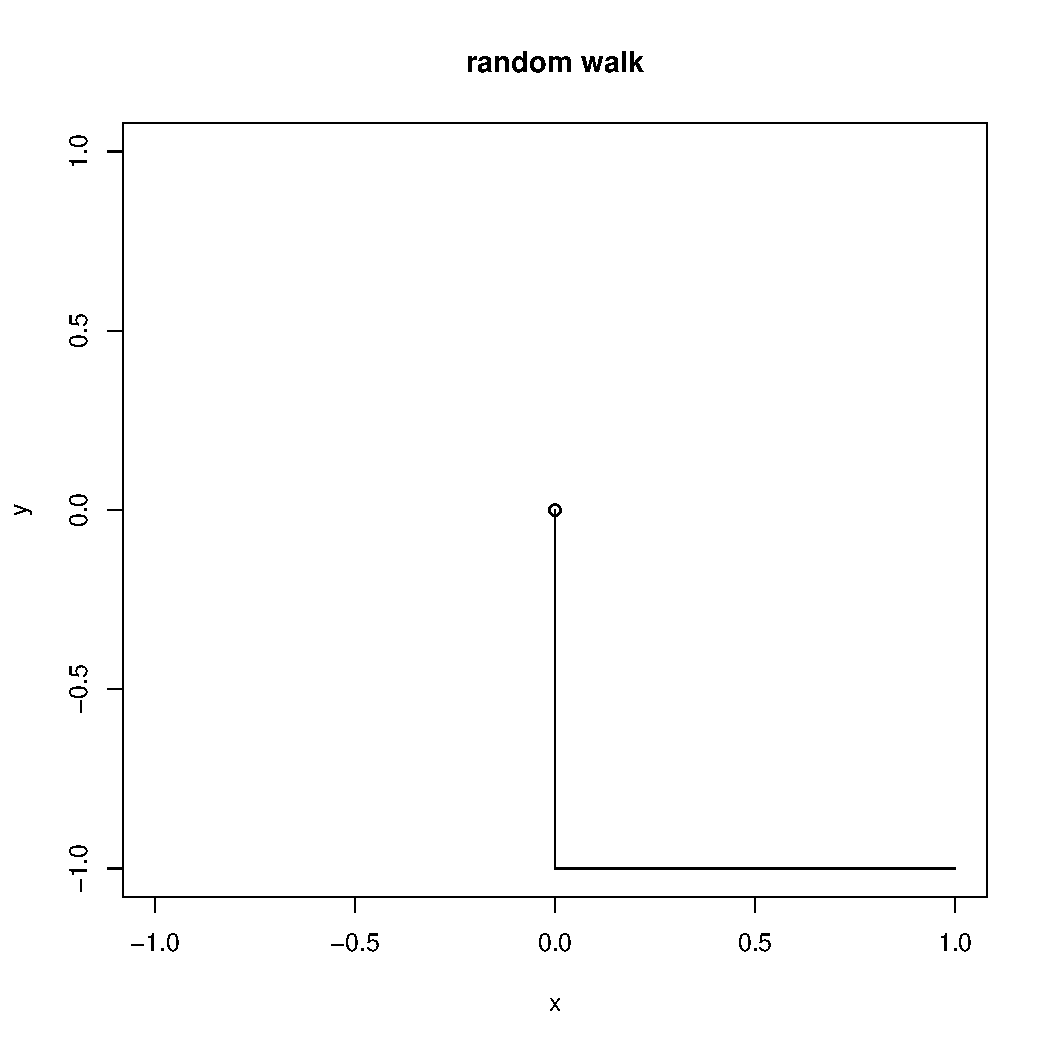
\includegraphics[width=\maxwidth]{figure/plot-1} 

\end{knitrout}

\\[ operator tells you the ith position of the walk
\begin{knitrout}
\definecolor{shadecolor}{rgb}{0.969, 0.969, 0.969}\color{fgcolor}\begin{kframe}
\begin{alltt}
\hlcom{# operator overloading}
\hlstr{'[.rm'} \hlkwb{<-} \hlkwa{function}\hlstd{(}\hlkwc{obj}\hlstd{,}\hlkwc{istep}\hlstd{)\{}
  \hlkwd{return}\hlstd{(obj}\hlopt{$}\hlstd{path[istep,])}
\hlstd{\}}
\hlstd{aWalk[}\hlnum{2}\hlstd{]}
\end{alltt}
\begin{verbatim}
## [1]  0 -1
\end{verbatim}
\end{kframe}
\end{knitrout}

At last, a start method to change the the origin
\begin{knitrout}
\definecolor{shadecolor}{rgb}{0.969, 0.969, 0.969}\color{fgcolor}\begin{kframe}
\begin{alltt}
\hlstr{'start<-'} \hlkwb{<-} \hlkwa{function}\hlstd{(}\hlkwc{x}\hlstd{,} \hlkwc{...}\hlstd{)} \hlkwd{UseMethod}\hlstd{(}\hlstr{"start<-"}\hlstd{)}
\hlstr{'start<-.rm'} \hlkwb{<-} \hlkwa{function}\hlstd{(}\hlkwc{obj}\hlstd{,} \hlkwc{value}\hlstd{)\{}
  \hlstd{obj}\hlopt{$}\hlstd{origin} \hlkwb{=} \hlstd{value}
  \hlstd{obj}\hlopt{$}\hlstd{path[}\hlnum{1}\hlopt{:}\hlstd{(obj}\hlopt{$}\hlstd{step}\hlopt{+}\hlnum{1}\hlstd{),]} \hlkwb{=} \hlstd{obj}\hlopt{$}\hlstd{path[}\hlnum{1}\hlopt{:}\hlstd{(obj}\hlopt{$}\hlstd{step}\hlopt{+}\hlnum{1}\hlstd{),]} \hlopt{+} \hlstd{value}
  \hlkwd{return} \hlstd{(obj)}
\hlstd{\}}
\hlkwd{start}\hlstd{(aWalk)} \hlkwb{<-} \hlkwd{c}\hlstd{(}\hlnum{5}\hlstd{,}\hlnum{7}\hlstd{)}
\hlstd{aWalk}
\end{alltt}
\begin{verbatim}
## Random Walk, Start at ( 5 7 ), after 2 steps, arrive final position at( 6 6 )
\end{verbatim}
\end{kframe}
\end{knitrout}
 

\textit{* R code saved in HW3.R; all codes have been run and tested}    

\end{document}
